\documentclass[preprintnumbers,amsmath,amssymb,superscriptaddress,twocolumn,showpacs]{revtex4-2}
\usepackage{graphicx}% Include figure files
\usepackage{dcolumn}% Align table columns on decimal point
\usepackage{bm}% bold math
\usepackage{natbib}
\usepackage{physics}
\usepackage[caption=false]{subfig}



%\newcommand{|}{Y$_2$SiO$_5$}
\def\sgn{\mathop{\rm sgn}}
\newcommand{\be}{\begin{equation}}
\newcommand{\ee}{\end{equation}}
\newcommand{\bea}{\begin{eqnarray}}
\newcommand{\eea}{\end{eqnarray}}

\begin{document}

\title{Low magnetic field depolarization of NV$^-$ centers through dipole-dipole interaction}

\author{C. Pellet-Mary$^1$, M. Perdriat$^1$, P. Huillery$^?$,  G. H\'etet} 

\affiliation{Laboratoire De Physique de l'\'Ecole Normale Sup\'erieure, \'Ecole Normale Sup\'erieure, PSL Research University, CNRS, Sorbonne Universit\'e, Universit\'e Paris Cit\'e , 24 rue Lhomond, 75231 Paris Cedex 05, France.}

\begin{abstract}
C'est trop bien
\end{abstract}

\maketitle

\begin{figure}
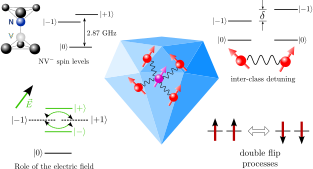
\includegraphics[width=0.45\textwidth]{Figures/shema_summary}
\caption{Shema}
\label{PL_NV_density}
\end{figure}

Intro

\begin{figure}
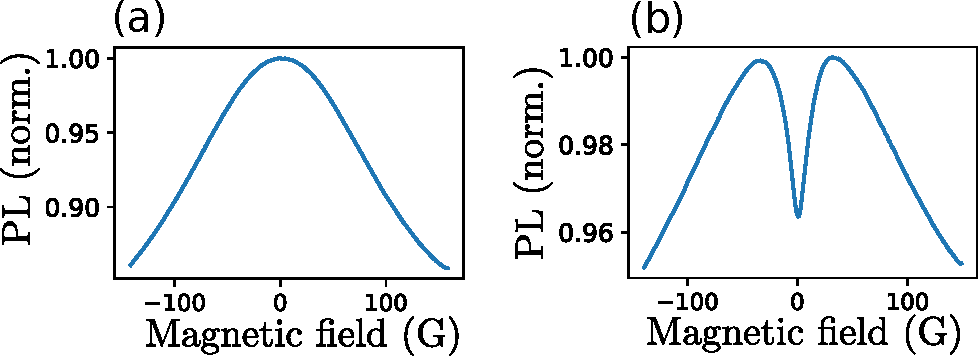
\includegraphics[width=0.45\textwidth]{Figures/fig dense vs pas dense}
\caption{Photoluminescence measurement from NV centers ensemble as a function of an external magnetic field randomly oriented (a) for a CVD sample containing $\approx$ 4 ppb NV$^-$ centers, (b) for an HPHT sample containing $\approx$ 3 ppm NV$^-$ centers}
\label{PL_NV_density}
\end{figure}

%In this letter/article, we characterize the depolarization of the spins observed for dense ensemble of NV centers in zero magnetic field and its potential application for DC magnetometry. While the main mechanism behind the depolarization, the lift in the degeneracy between the four classes of NV centers, is already well studied and can be exploited in a microwave-less vector magnetometry protocol, we found two other depolarization mechanisms specific to the zero-field region which could play an important role in a low-field magnetometry protocol.
%
%The main signature of the spin depolarization in low field is the characteristic dip in photoluminescence (PL) observed only for high density ($\gtrsim 1$ ppm) of NV centers, as shown on fig \ref{PL_NV_density}. The decrease in the spins' lifetime in zero field makes the optical polarization scheme of the NV centers less effective and therefore reduce the population of the bright $\ket{0}$ spin state. %The reason for the decrease in PL at higher magnetic field values is the mixing of the bright spin state $\ket{0}$ to the darker state $\ket{-1}$ induced by the transverse magnetic field. This effect does not modify (on first approximation) the spins' lifetime, and is common to both dense and sparse samples.

Fig. \ref{PL_NV_density} shows the change in photoluminescence (PL) with respect to an external magnetic field for two samples with a low and high concentration of NV$^-$ centers. Both samples show a decrease in PL as the magnetic field amplitude increases, due to eigenstate mixing caused by the transverse part of the magnetic field \citep{epstein2005anisotropic,lai2009influence}. We notice however a stark difference in the low magnetic field region where only the high-density sample observe a drop in PL. In this article we propose to explore the reasons behind this zero-field line present only for dense NV$^-$ ensemble.

Unlike the decrease in PL for higher magnetic field values, the drop in PL at low magnetic field is associated with a decrease of the NV's spin lifetime $T_1$. Indeed, since the $\ket{m_s=0}$ spin state is brighter than the $\ket{m_s=\pm 1}$ states, and since the optical pumping in the $\ket{m_s=0}$ state is in competition with the relaxation in a thermal distribution of the states, decreasing the spins lifetime results in a decrease of the NV PL \citep{finco2021imaging}. To understand the behavior of the PL in zero-field, we therefore need to study the dynamics of the spin in the low magnetic field region.

\begin{figure}
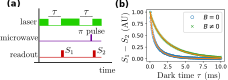
\includegraphics[width=0.45\textwidth]{Figures/fig T1}
\caption{Spin $T_1$ measurement protocol. (a) Sequence used to measure the spin lifetime : the laser is turned off for a time $\tau$ twice and the spin state is read at the end of the dark time by measuring the initial photoluminescence when the laser is turned back on. A microwave $\pi$-pulse resonant with one of the spin transition is placed before the second reading. The  $T_1$ sequence result is the subtraction $S_1-S_2$. (b) Measurement of $S_1-S_2$ for a high density of NV centers in zero magnetic field field and non-zero magnetic field. The fit (orange plain line) is detailed in the main text}
\label{T1}
\end{figure}

The $T_1$ depolarization dynamics of single or dilute NV centers at room temperature is dominated by a two-phonon Raman process \citep{redman1991spin,jarmola_temperature-_2012,norambuena2018spin}, which depends on the crystal lattice temperature but does not depend on the external magnetic field. However, it has been observed that dense NV centers ensemble have an additional spin decay channel \citep{jarmola_temperature-_2012,jarmola_longitudinal_2015,mrozek_longitudinal_2015, choi_depolarization_2017, akhmedzhanov_microwave-free_2017, akhmedzhanov_magnetometry_2019, pellet2021magnetic, mrozek2021characterization}, which depends greatly on the magnetic field and not on the temperature . This effect has been attributed to cross-relaxation between the NV centers through dipole-dipole coupling \citep{mrozek_longitudinal_2015, choi_depolarization_2017}. Some inhomogeneity between the NV centers is further needed in order to explain the depolarization of the spin ensemble. We will denote $T_1^{\rm ph}$ the characteristic time associated with the phonon relaxation process and $T_1^{\rm dd}$ the characteristic time associated with the dipole-dipole relaxation process.

The spin lifetime protocol used here is described in Fig. \ref{T1} and is based on previous similar experiments \citep{jarmola_temperature-_2012, mrozek_longitudinal_2015, choi_depolarization_2017}. It consists in a pump-probe measurement where the spins are first polarized in the $\ket{0}$ state by a green laser, and read-out optically after a variable dark time $\tau$. Using only this sequence can result in artifacts in the signal, mostly due to charge state transfer in the dark \citep{giri_coupled_2018, giri_selective_2019}. It is therefore convenient to repeat the sequence with an additional $\pi$ pulse right before the spin read-out to project the remaining $\ket{0}$ polarization into a darker $\ket{+1}$ or $\ket{-1}$ state. By subtracting the result of the two sequences, we select only the spin-dependent part of the signal, with the added benefit of being able to select a specific class of NV centers. 

\begin{figure*}
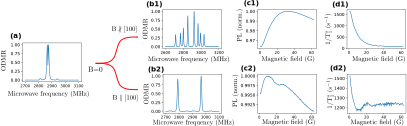
\includegraphics[width=.95\textwidth]{Figures/fig 100 vs 1x1x1x1}
\caption{Dependency on the magnetic field angle for the zero field depolarization. (a) ODMR spectrum in zero field. (bi) ODMR spectrum for a magnetic field $\approx$ 60 G, misaligned by $\sim  24^\circ$ with the [100] axis. (bii) Normalized photoluminescence of the NV$^-$ ensemble as a function of the magnetic field amplitude. (biii) Stretch part of the spin decay $1/T_1^{\rm dd}$ as a function of the magnetic field amplitude. (ci), (cii) and (ciii) : same measurement with a magnetic field aligned with the [100] axis}
\label{100_VS_1x4}
\end{figure*}

The ensemble spin decay is non-exponential due to inhomogeneities between the NV$^-$ centers. We will base our interpretations of the experimental results on the NV-fluctuator model developed in \citep{choi_depolarization_2017}. A conclusion of this model is that, for an homogeneous 3D distribution of fluctuator, the dipole-induced lifetime should be stretched-exponential with a stretch factor $\beta=1/2$. Such an ensemble lifetime is indeed observed when $T_1^{\rm dd} \ll T_1^{\rm ph}$  (see SI).

For the samples used in this paper (detailed in SI), we observed that $T_1^{\rm dd} \sim T_1^{\rm ph}$, meaning that we had to include both  in our analysis. The resulting fitting formula is therefore :
\begin{equation}
S(\tau)=A \exp (-\frac{\tau}{T_1^{\rm ph}} -\sqrt{\frac{\tau}{T_1^{\rm dd}}}),
\end{equation}
Further details on the fitting procedure are available in SI. For the rest of the article we will be only interested on the stretched exponential lifetime ${T_1^{\rm dd}}$.

%\begin{figure}
%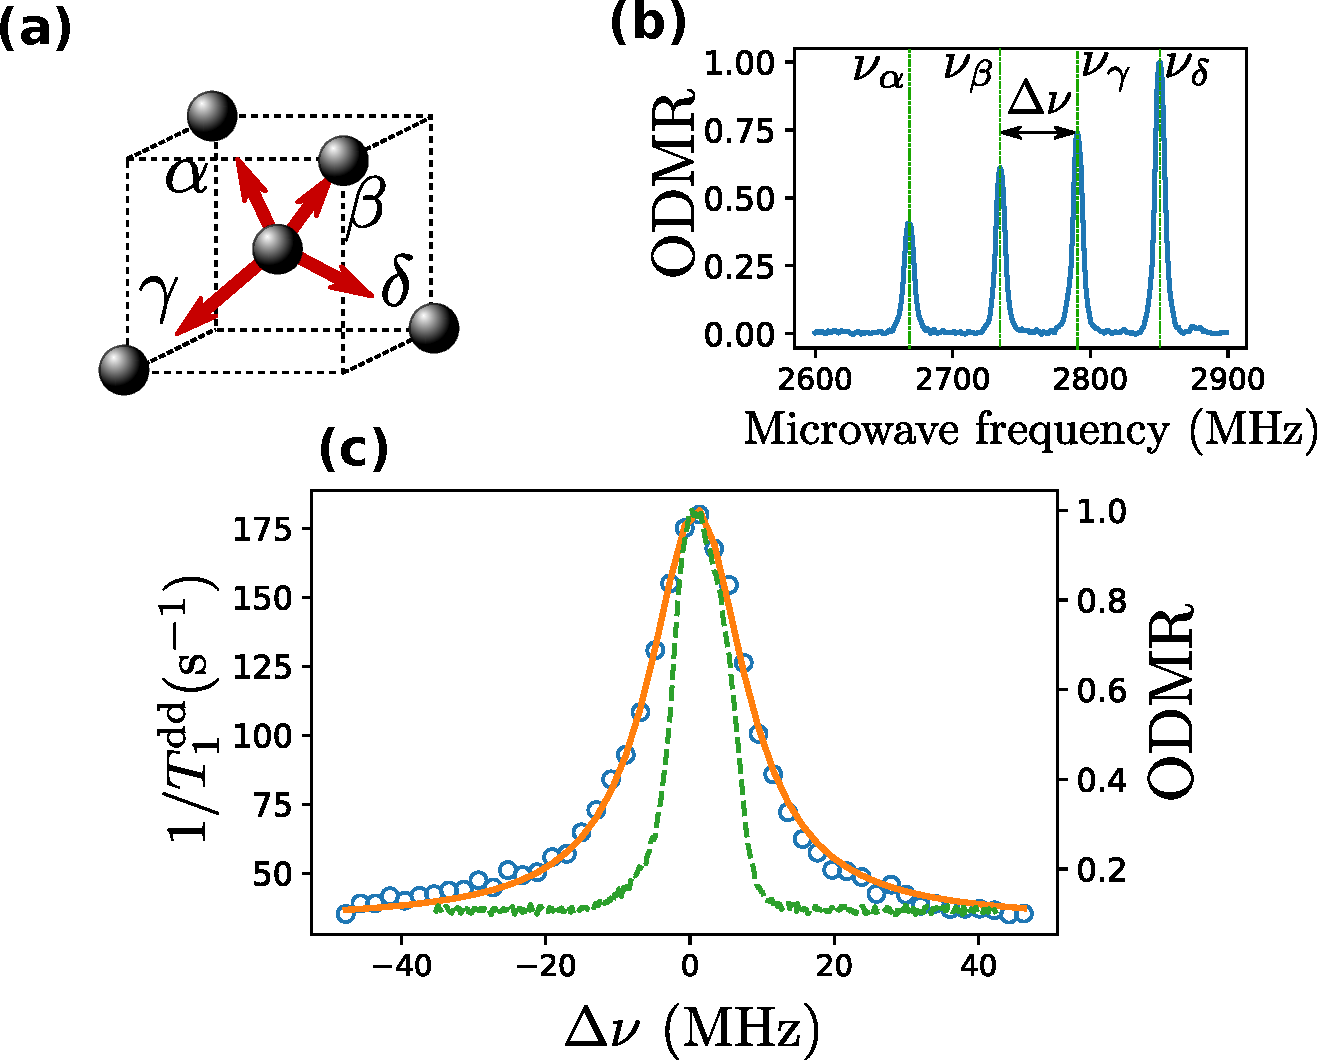
\includegraphics[width=0.45\textwidth]{Figures/fig largeur fluct}
%\caption{Tuning resonant coupling through magnetic field orientation. (a) Sketch of the four possible orientations ("classes") in a single crystal diamond lattice. (b) ODMR spectrum showing four $\ket{0} \to \ket{-1}$ resonances corresponding to the four spin classes. The detuning $\Delta \nu$ between the classes $\beta$ and $\gamma$ was controlled by changing the orientation of the external magnetic field.(c) Stretch part of the lifetime decay for the spins resonant with $\nu_\gamma$ as a function of the detuning $\Delta \nu$ (blue circles), fitted by a Lorentzian with half width at half maximum 8.04 MHz . Green dashed line correspond to the ODMR width of a single class stretched by a factor $\sqrt 2$, approximating the overlap of the two classes (see SI).}
%\label{largeur_fluct}
%\end{figure}

%Fig. \ref{largeur_fluct} illustrates how we can use the NV center geometry to tune the resonant dipolar-coupling between the spins. Because of the diamond symmetry, we can distinguish 4 groups ("classes") of NV centers, based on the four possible orientation of the NV axis in the crystal. These four classes have \textit{a priori} different spin resonance frequency based on the projection of the magnetic field on their respective NV axis. By tuning the angle of the magnetic field, we can therefore control the frequency detuning between the different classes, and as a result we can control the number of resonant NV centers by bringing in and out of resonance several classes.
%
%Fig. \ref{largeur_fluct} (c) in particular shows the dipole-induced lifetime $T_1^{\rm dd}$ for a given class as a function of the energy detuning with another class. One can notice that the width of the $T_1^{\rm dd}$ bell shape is significantly larger than that of the frequency overlap between the two classes, modeled here by an ODMR line stretched by a factor $\sqrt{2}$ (see SI). This extra width can not be attributed to the dipole-dipole coupling strength : for a 3 ppm concentration of NV$^-$ centers, the average coupling strength between neighboring NV centers should be $\sim 27\ \rm kHz$, two order of magnitude below the observed width. We can also see that $T_1^{\rm dd}$ follows a Lorentzian shape despite the ODMR lines being non-Lorentzian. These two observations corroborate the idea developed in \cite{choi_depolarization_2017} that the interaction width is dominated by the noise spectrum of the lifetime-limited fluctuators.



One of the way we can isolate dipole-dipole related phenomena with NV centers is by tuning the number of NV centers resonant with each other. Indeed, Fig. \ref{100_VS_1x4} (bi) shows the characteristic 8 lines observed with ensemble NV optically detected magnetic resonance (ODMR) spectrum. These 8 lines correspond to the four "classes" of NV centers - that is physical orientation of the NV axis is the diamond crystal cell - multiplied by the two possible spin transitions $\ket{0}\to\ket{-1}$ and $\ket{0}\to\ket{+1}$. The transitions of the four different classes can be controlled somewhat independently by changing the amplitude and orientation of the external magnetic field, and in particular they can be brought to resonance for particular orientation of the magnetic field. Fig. \ref{100_VS_1x4} (ci) shows an example where all four classes are brought to resonance by placing the magnetic field along the [100] crystalline axis. Other example of class resonance are given in SI.

Fig. \ref{100_VS_1x4} (bii) and (biii) shows respectively the PL and the stretched exponential spin decay $T_1^{\rm dd}$ of an ensemble of NV centers with respect to the amplitude of the external magnetic field. The orientation of the magnetic field was chosen in order to lift the degeneracy between the four classes, as shown in Fig. \ref{100_VS_1x4} (bi). We observe that the drop in PL at low magnetic field is indeed correlated with an increase in the spin decay rate, as is expected due to the higher number of resonant spins in zero magnetic field, where all four classes are resonant, compared to the non-degenerate case for $\vec \neq 0$. We can also see that the decrease in PL for $B>40\ \rm G$ due to state mixing by the transverse magnetic field is not correlated to a modification of the spin lifetime.

However, the splitting of the four classes is not sole reason to the decrease of the spin lifetime in low magnetic field. Indeed, we performed similar measurements in Fig. \ref{100_VS_1x4} (cii) and (ciii) but this time fixing the magnetic field orientation along the [100] axis. For this particular orientation, the four classes are always resonant, regardless of the field amplitude. We can see that, although considerably reduced, there still is an increase in the spin decay rate and a corresponding drop in PL for low magnetic field values. We attribute the slight drop in PL and the corresponding bump for $1/T_1^{\rm dd}$ at $B \sim 20\ \rm G$ to dipolar interaction with NV having a first neighbor $^{13}C$ \cite{pellet2021optical}.

The aim of this paper is to understand the remaining contribution to the spin decay in this second case. We identified and isolated two additional effects : the domination by the local electric field for low magnetic field value which results in a change of the spin Hamiltonian eigenstates, and the presence of double-flip processes where both NV spins involved in the dipole-dipole coupling flip their spin in the same direction.

In order to distinguish these two contributions, we decided to simulate the effect of the electric field by using a transverse magnetic field : for relatively weak transverse magnetic field, the eigen basis of the spin Hamiltonian is close to $\{ \ket{0},\ket{+}=\frac{\ket{+1}+\ket{-1}}{\sqrt{2}},\ket{-}=\frac{\ket{+1}-\ket{-1}}{\sqrt{2}} \} $, which is the the spin Hamiltonian basis when the electric field dominates, as detailed in SI. This property has been used to observe a linear dependence in the electric field for the spin transition frequencies by applying an external transverse magnetic field \cite{dolde2011electric,qiu2022nanoscale}.

\begin{figure}
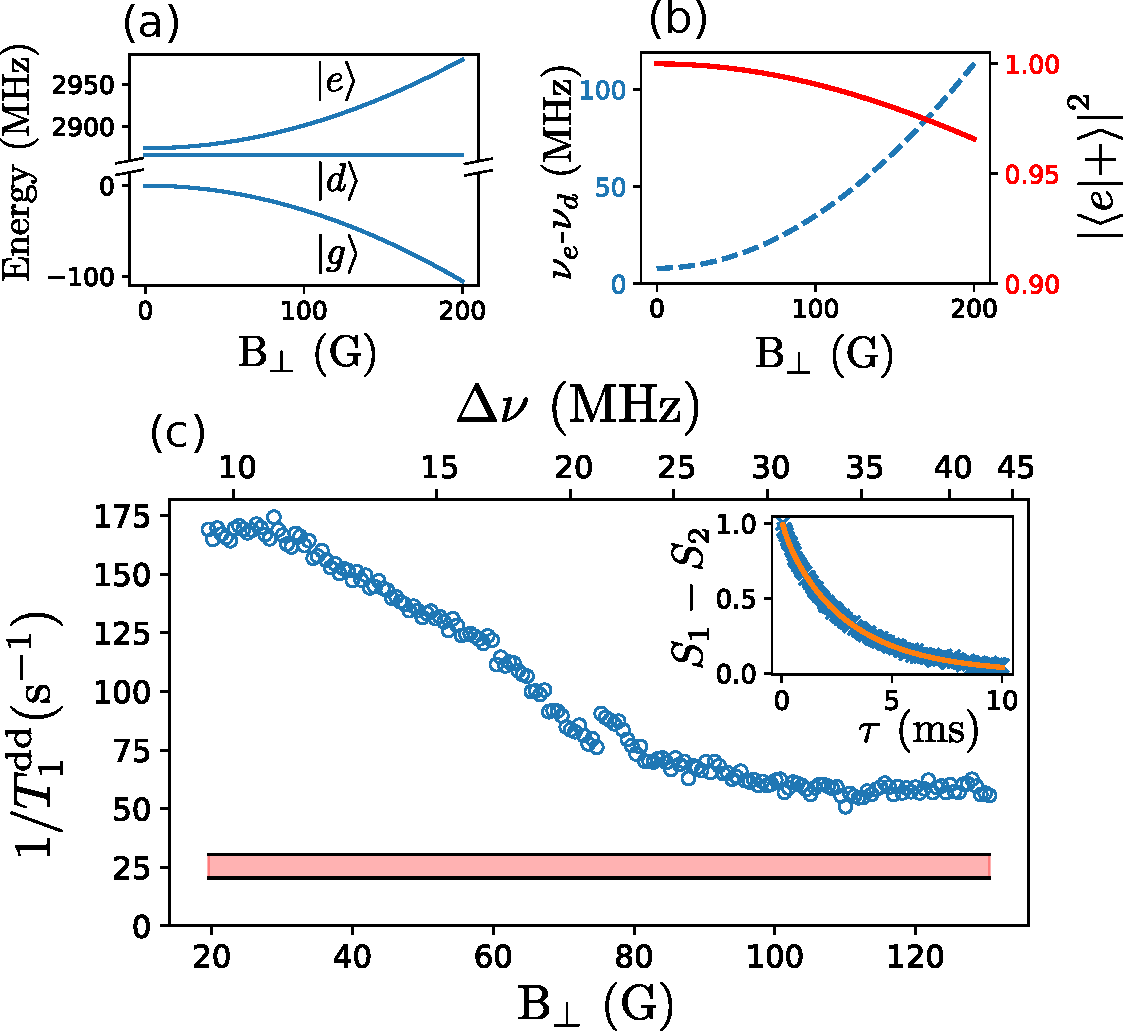
\includegraphics[width=0.45\textwidth]{Figures/fig transverse field V2}
\caption{(a) Simulated energies for the spin Hamiltonian in the presence of pure transverse magnetic field $B_\perp$. The three spin levels are denoted $\ket{g}$, $\ket{d}$ and $\ket{e}$. (b) Blue dashed curve : frequency detuning $\Delta \nu$ between the $\ket{g}$, $\ket{d}$ states. Red plain curve : Matching factor $\abs{\bra{e}\ket{+}}^2$ between the states $\bra{e}$ and $\bra{+}$. (c) Measurement of the stretched exponential decay rate $1/T_1^{\rm dd}$ for a single class as a function of the measured detuning $\Delta \nu$ between the two transitions $\ket{g} \to \ket {d}$ and  $\ket{g} \to \ket {e}$ for purely transverse magnetic field. The green dashed line correspond to the decay rate for the same class when the magnetic field is longitudinal}
\label{B_transverse}
\end{figure}

Fig. \ref{B_transverse} (a) shows the energy levels for the three eigenstates of the NV spin Hamiltonian with respect to a purely transverse magnetic field. We will denote these eigenstates in the general case $\ket{g}$, $\ket{d}$ and $\ket{e}$. For weak transverse magnetic field, $\ket{g} \approx \ket{0}$, $\ket{d}=\ket{-}$ and $\ket{e} \approx \ket{+}$. As the magnetic field increases, $\ket{g}$ and $\ket{e}$ starts to become a mixing of $\ket{0}$ and $\ket{+}$ while $\ket{d}$ remains equal to $\ket{-}$.

Crucially, this mixing happens on a different scale than the associated energy splitting of the $\ket{d}$ and $\ket{e}$ states : Fig. \ref{B_transverse} (b) shows both the splitting between the energy levels of $\ket{d}$ and $\ket{e}$, and the matching factor $\abs{\bra{e}\ket{+}}^2$ characterizing the closeness of the states $\bra{e}$ and $\bra{+}$. We can see that for a field value of $\sim 130 G$, the splitting between the $\ket{d}$ and $\ket{e}$ reaches $\sim 50 MHz$, far exceeding the range of the dipole-dipole resonant coupling (see details in SI), but $\abs{\bra{e}\ket{+}}^2 > 0.98$ meaning that the spin Hamiltonian eigenstates are still roughly in the $\ket{0}, \ket{+}, \ket{-}$ basis. We can therefore decouple the effects of the double-flip processes, which are no longer resonant, from the effects of the change of basis induced by the transverse electric - or in this case magnetic - field.

Fig. \ref{B_transverse} (c) shows the measurement of the stretched lifetime $T_1^{\rm dd}$ for a single class of NV centers exposed to a transverse magnetic field between 25 and 130 G. The detuning $\Delta \nu$ between the two states $\ket{d}$ and $\ket{e}$ was measured through ODMR. We attribute the decrease in the spin decay rate when the detuning increases to the loss of effectiveness of the double-flip processes. We can notice that the decay rate reaches a plateau for $\Delta \nu \geq 30\ \rm MHz$ with a value about twice as big as the decay rate for a longitudinal magnetic field. This plateau we attribute to the effect of the transverse magnetic field, which we assume to be similar to the effect of the electric field in the low magnetic field regime. We should note that the effect of the double-flip processes is about 4 times more important in the depolarization rate than the effect of the electric field, even though the states are not initially fully resonant.

Overall we predicted, based on an extension of the fluctuator model developed in SI, an increase by a factor of $\sim 4$ of the dipole-dipole induced decay rate in the non-magnetic basis $\ket{0}, \ket{+}, \ket{-}$ compared to the magnetic basis $\ket{0}, \ket{+1}, \ket{-1}$. While the measured increase is smaller than the predicted one, as with most of the predictions based on the fluctuator model, the measurements agrees with the theoretical increase in the flip-flop rate in the $\ket{+/-}$ basis compared to the $\ket{\pm 1}$ basis.

Similarly, we can compute the predicted decay rate in the $\vec B \parallel \left[100\right]$ case compared to the $\vec B = 0$ case, and find a theoretical increase of $\sim 20\%$ in the $\vec B = 0$ case due to the effects of the local electric field. This, along with the double-flip processes explains the behavior observed in Fig. \ref{100_VS_1x4} (cii) and (ciii).

%... (lis un peu ce que t'as déja écrit avant de tout réécrire, je te connais moi futur. En vrai c'est de la merde, j'ai tout réécrit)
%The dipole-dipole interaction Hamiltonian between two spins ${\vec S}_1$ and ${\vec S}_2$ reads :
%\begin{equation}
%\mathcal{H}^{\rm dd}= -\frac{J_0}{r^3}\left(3\left({\vec S}_1 \cdot \vec u \right)\left({\vec S}_2 \cdot \vec u \right) - {\vec S}_1 \cdot {\vec S}_2  \right),
%\end{equation}
%Where $J_0= (2 \pi) 52\ \rm MHz \cdot \rm{nm}^3$, $\vec r$ is the relative positions of the two spins and $\vec u = \frac{\vec r}{\norm{\vec r}}$. In situations such as the one described in Fig. \ref{largeur_fluct}, the only relevant terms of $\mathcal{H}^{\rm dd}$ in term of population transfer are the flip-flop terms such as $\mel{0,+1}{\mathcal{H}^{\rm dd}}{+1,0}$. In zero magnetic field however, we have to take into account other aspects of the dipolar Hamiltonian in consideration.
%
%First is the change of basis of the single spin Hamiltonian $\mathcal{H}_s$ : in zero external magnetic field, the eigenstates of $\mathcal{H}_s$ in the $\{\ket{+1},\ket{-1}\}$ manifold are determined by local electric and magnetic field coming from nearby impurities \cite{mittiga2018imaging}. For the samples used in this study, $\mathcal{H}_s$ was dominated by local electric field (see SI), meaning that the proper eigenstates of $\mathcal{H}_s$ in zero magnetic field are $\{ \ket{0},\ket{+}=\frac{\ket{+1}+\ket{-1}}{\sqrt{2}},\ket{-}=\frac{\ket{+1}-\ket{-1}}{\sqrt{2}} \} $
%
%Because the splitting between $\ket{+}$ and $\ket{-}$ ($\approx 9\ \rm MHz$) is much greater than the dipole-dipole interaction ($J_0 / r^3 \approx 30\ \rm kHz$), the flip-flop terms of $\mathcal{H}^{\rm dd}$ now reads $\mel{0,+}{\mathcal{H}^{\rm dd}}{+,0}$. Averaging over all relative positions of two aligned NV centers, we found that on average $\abs{\mel{0,+}{\mathcal{H}^{\rm dd}}{+,0}}$ was greater than 
%$\abs{\mel{0,+1}{\mathcal{H}^{\rm dd}}{+1,0}}$ by a factor $1.8 \sim 2$ depending on the correlation lengths of the local electric field.
%When all four classes are resonant, the theoretical decrease in the spin lifetime due to the change of basis is $\sim 20 \%$ (See SI de ouf).
%
%Second is the near-resonance condition of the double-flip processes such as $\mel{0,+1}{\mathcal{H}^{\rm dd}}{-1,0}$ or $\mel{0,+}{\mathcal{H}^{\rm dd}}{-,0}$. These terms usually couple non resonant states due to the energy mismatch between $\ket{+1}$ and $\ket{-1}$. However in zero field, the energy splitting between $\ket{+}$ and $\ket{-}$ is comparable with the fluctuator's spectral width measured in Fig. \ref{largeur_fluct} to be $\approx 8\ \rm MHz$, making the double-flip population transfer possible.
%
%\begin{figure}
%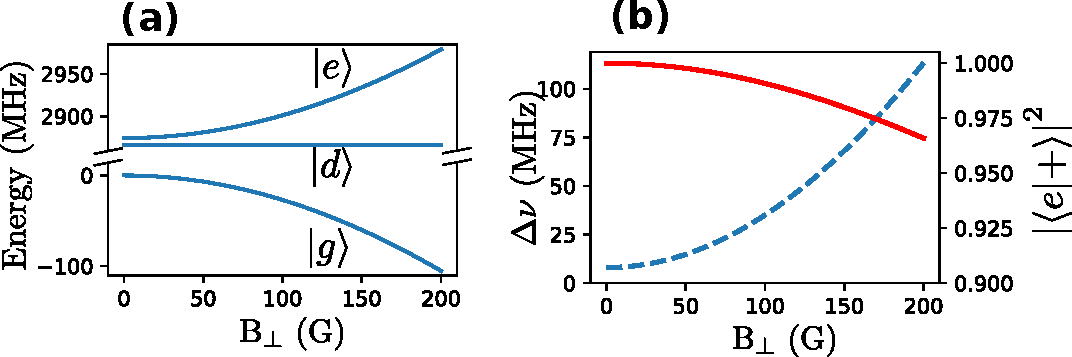
\includegraphics[width=0.45\textwidth]{Figures/fig transverse field simu}
%\caption{Simulated eigenstates of the spin Hamiltonian in the presence of purely transverse magnetic field. (a) Energies of the three eigenstates $\ket{g}$, $\ket{d}$ and $\ket{e}$ as a function of the magnetic field amplitude. (b) Blue dashed curve : frequency detuning between the two transitions $\ket{g} \leftrightarrow \ket{d}$ and $\ket{g} \leftrightarrow \ket{e}$. Plain red curve : projection of $\ket{e}$ on $\ket{+}=(\ket{+1}+\ket{-1})/\sqrt{2}$ as a function the magnetic field. Is equal to the projection of $\ket{g}$ on $\ket{0}$.}
%\label{calculs_B_transverse}
%\end{figure}
%
%In order to evaluate the relative contribution of these two factors, we investigate the spin relaxation in the case of pure transverse magnetic field. Calling $\{ \ket{g}, \ket{d}, \ket{e} \}$ the three eigenstates of the spin Hamiltonian in the presence of purely transverse magnetic field, Fig. \ref{calculs_B_transverse} shows that for small enough magnetic field, the $\{ \ket{g}, \ket{d}, \ket{e} \}$ basis is almost equal to the $\{ \ket{0},\ket{+},\ket{-} \} $ basis : for $B=120\ \rm G$, $\braket{0}{g}\approx 0.99$, $\braket{-}{d}=1$ and $\braket{+}{e}\approx 0.99$. However the energy difference between $\ket{d}$ and $\ket{e}$ reaches $\approx 45\ \rm G$ which is high enough to cancel out the double-flip processes and allows us to isolate the change of basis hypothesis from the double-flip one.
%%As shown in Fig. SOON, (and in SI), the $\{ \ket{0},\ket{+},\ket{-} \} $ basis correspond to the spin Hamiltonian eigenstates in two situations : either in zero magnetic field when the electric field dominates, or when the magnetic field is purely transverse, as long as it remains small before the zero-field splitting. %(rq : est-ce que je dois mettre le hamiltonien de spin dans le main text du coup ?).
%
%\begin{figure}
%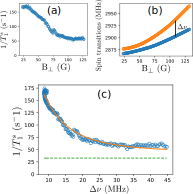
\includegraphics[width=0.45\textwidth]{Figures/fig transverse field}
%\caption{Modification of the stretch lifetime in the presence of purely transverse magnetic field. (a) Stretch component of the ensemble lifetime as a function of the field amplitude. (b) Transition frequencies for the $\ket{g} \leftrightarrow \ket{d}$ and $\ket{g} \leftrightarrow \ket{e}$ transitions, measured through ODMR. (c) Stretch component of the lifetime as a function of the frequency detuning between the two transistions (blue circles), fitted by a Lorentzian centered in $\Delta \nu=0$ with half width at half maximum 8MHz. The green dashed line correspond to the lifetime of a single class aligned with the magnetic field.}
%\label{exp_B_transverse}
%\end{figure}
%
%Fig. \ref{exp_B_transverse} shows the dipole-dipole spin relaxation $T_1^{\rm dd}$ for a class of NV whose axis is orthogonal to the applied magnetic field. By monitoring the frequencies of the transitions $\ket{g} \leftrightarrow \ket{d}$ and $\ket{g} \leftrightarrow \ket{e}$, we can deduce the detuning $\Delta \nu$ between the two-spin states $\ket{0,+}$ and $\ket{-,0}$. Plotting then $1/T_1^{\rm dd}$ as a function of $\Delta \nu$, we can notice two things. 
%
%First the decrease of $1/T_1^{\rm dd}$ as $\Delta \nu$ increases which corresponds to the loss in effectiveness of the double flip processes. The shape of the curve matches decently well with the tail of a Lorentzian centered in $\Delta \nu=0$ with a width of 8 MHz, confirming that the double-flip process interaction range is likely determined by the fluctuators noise spectrum just like the flip-flop processes. 
%
%Second is the plateau reached for $\Delta \nu \gtrsim 30\ \rm MHz$. The final $1/T_1^{\rm dd}$ value is about twice as high as that for a spin well aligned with the magnetic field, showing the increased depolarization due to the change of basis.
%
%This experiment shows that, for the sample studied here, the depolarization due to the double-flip processes dominates the one due to the change of basis in zero magnetic field.

\section*{Magnetometry}
\begin{figure}
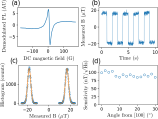
\includegraphics[width=0.45\textwidth]{Figures/fig_magneto}
\caption{Low field magnetometry protocol. (a) Demodulated photoluminescence as a function of an externally applied magnetic field with an additional oscillatory magnetic field. (b) Measured magnetic field when alternating a small external magnetic field offset. (c) Histogram of the measurement in Fig. (b) fitted with gaussians of standard deviation $\sigma=1.5\ \mu \rm T$. (d) Measured sensitivity as function of the angle between the external magnetic field and the [100] crystalline axis.}
\label{magneto}
\end{figure}
%
DC microwave-less magnetometry has already been performed with NV ensembles, using either NV-NV cross-relaxations \citep{akhmedzhanov_microwave-free_2017,akhmedzhanov_magnetometry_2019} or level anti-crossing \citep{Wickenbrock, zheng2017level, zheng_microwave-free_2020}. Here we propose to perform a similar protocol, but using the spin depolarization in zero-field. The main difference with the previously mentioned protocols is the fact that this one doesn't rely on crystalline orientation, making this protocol usable with diamond powders or polycrystalline samples. The idea of performing optical magnetometry on the zero-field photoluminescence feature of NV ensembles has been suggested before \cite{filimonenko2018weak, filimonenko2022manifestation} but had not been implemented so far.

Fig. \ref{magneto} (a) shows the demodulated PL when a DC magnetic field is scanned in a random direction and an additional alternating magnetic field of a few Gauss at $\sim \ \rm kHz$ is added through the same electromagnet (see experimental details in SI). We can see a sharp and relatively linear slope in low field $\abs{B} < 5\ \rm G$. Once calibrated, in this case with ODMR, the slope can provide a 1D magnetic field measurement, which could be extended to 3D with a set of 3 coils or 3 electromagnets, as seen in \cite{zheng_microwave-free_2020}.

In order to measure the sensitivity of the measurement, we alternate a small DC field of $\approx 40\ \mu\rm{T}$ every few seconds and take an histogram of the measured fields, as shown in Fig. \ref{magneto} (b) and (c). The histogram is well fitted with gaussians of standard deviation $\sigma=1.5\ \mu \rm T$. The measurement was performed here with an output low-pass filter of time constant $\tau=3\ \rm ms$, which allows us to measure the sensitivity $\eta=\sigma \sqrt{\tau}=82\ \rm{nT}/\sqrt{\rm Hz}$.

We can then try to measure the relative importance of the three causes of spin depolarization on the field sensitivity, namely the splitting of the classes, the local electric field and the double-flip processes. In order to do so, we measure the sensitivity while changing the angle of the field. When $\vec B$ is aligned with the [100] crystalline axis, only the double flips and the electric field cause a depolarization, whereas in every other orientation the three effects are at play.

The results are shown in Fig. \ref{magneto} (d). We can see a slight increase of $\sim$ 10\% in the sensitivity as we leave the [100] region, but overall the sensitivity remains relatively flat, which means that the double-flips and electric field effects are the dominant factors in the sensitivity of this protocol. While it may seem surprising that the effects with a lower contribution on the PL contrast have a higher effect on this PL-based protocol, what matters here is not the absolute contrast but the slope of the change of contrast with respect to the magnetic field, which is sharper for the electric field and double flips than it is for the lift of degeneracy. %This is in agreement with the measurements in Fig. \ref{100_VS_1x4} : even though the contrast is much better in the not-[100] case, the slope in term of contrast percentage/magnetic field is comparable in both cases (en faite pas complètement, y'a pas loin d'un facteur 2 sur les dérivées numériques)
It should be noted though that this observation is sample dependent, and that other samples, including from the same batch, have shown a higher orientation dependence, corresponding to a lower contribution from the electric field and double-flip processes.

\section*{Conclusion}
In this work we have identified three mechanisms causing the extra spin depolarization observed in zero field for dense ensemble of NV$^-$ centers, all related to an increase in the dipole-dipole cross-relaxations between the spins : the lift of degeneracy between the four classes caused by the magnetic field, the domination of the local electric field which causes a change in the Hamiltonian eigenstates, and the double-flip process allowed by the proximity in energy of the spin $\ket{\pm}$ states. We identified the lift in degeneracy as the main cause in the zero-field depolarization, followed by the double-flip processes and then the electric field. We have demonstrated a potential use of this depolarization as a DC microwave-less and orientation-free magnetometer with sensitivity below $100\ \rm{nm}/\sqrt{\rm Hz}$ for a single $10\ \mu \rm m$ crystal.We have observed that in some cases the double-flips and electric field play a more important role than the lift of degeneracy in the magnetometry sensitivity.
\section*{acknowledgements}

\bibliographystyle{plain}
\bibliography{CR}{}



\end{document}